\documentclass[10 pt,usenames,dvipsnames, oneside]{article}
\usepackage{../../../modelo-ensino-medio}



\begin{document}

\begin{center}
  \begin{minipage}[l]{3cm}

\includegraphics[width=2cm]{logo}    
\end{minipage}\hfill
\begin{minipage}[r]{.8\textwidth}
 {\Large \scshape Atividade: Analgésicos}  
\end{minipage}
\end{center}
\vspace{.2cm}

\ifdefined\prof
%Habilidades da BNCC
\begin{objetivos}
\item \textbf{EM13MAT304} Resolver e elaborar problemas com funções exponenciais nos quais é necessário compreender e interpretar a variação das grandezas envolvidas, em contextos como o da Matemática Financeira e o do crescimento de seres vivos microscópicos, entre outros. 
\end{objetivos}

%Caixa do Para o Professor
\begin{goals}
%Objetivos específicos
\begin{enumerate}
\item Modelar situações (dadas verbalmente, em tabelas ou gráficos) de decaimento exponencial.
\end{enumerate}

\tcblower

%Orientações e sugestões
\begin{itemize}
\item Caso haja dificuldade de acesso a internet, considere em seu planejamento solicitar aos estudantes que já tragam de casa a informação referente a meia-vida de três analgésicos. Alternativamente você pode oferecer essa informação, neste endereço há uma lista com diversos medicamentos e suas meia-vidas.  
\url{https://sbgg.org.br/wp-content/uploads/2016/06/farmacocinetica-dos-medicamentos.pdf}

\item Curiosamente um analgésico bastante conhecido e para o qual não há conclusão científica sobre a sua meia-vida no organismo humano é a Dipirona.
\end{itemize}
\end{goals}

\bigskip
\begin{center}
{\large \scshape Atividade}
\end{center}
\fi

Todo medicamento é acompanhado por uma bula, que contém, entre outros tópicos, a composição, informações ao paciente, informações técnicas e posologia. Uma informação técnica importante é a meia-vida do medicamento, que indica o tempo em que o mesmo se reduz a $50\%$ do que tinha no organismo do paciente, após a introdução do medicamento. O tempo de meia-vida dos medicamentos possibilita uma estimativa da duração do efeito farmacológico, sendo assim um importante parâmetro para médicos e também para a indústria farmacêutica.

\begin{enumerate}

\item{} Descubra quais são os três analgésicos mais conhecidos entre os seus colegas de turma.

\item {} Faça uma pesquisa na internet e descubra as meias-vidas dessas substâncias. Use as palavras-chaves: farmacocinética, meia-vida, semivida, farmacodinâmica.

\item {} Para cada uma delas, escreva a expressão da função exponencial que modela a quantidade de substância no sangue em função do tempo.

\item{} O gráfico abaixo representa a quantidade em $mg$ de um antibiótico no sangue de um paciente durante 24 horas. Descreva a dosagem, a meia-vida e a posologia do medicamento para esse paciente.

\end{enumerate}

\begin{figure}[H]
\centering
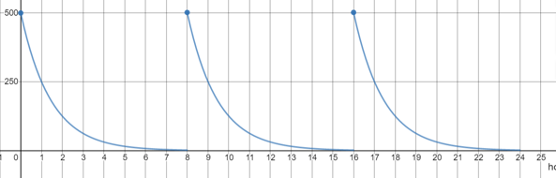
\includegraphics[width=.8\linewidth]{antibioticos.png}
\end{figure}

\ifdefined\prof
\begin{solucao}

\begin{enumerate}
\item Resposta pessoal.

\item ACETAMINOFENO (PARACETAMOL) ME Via Oral (VO): 4h

ÁCIDO ACETILSALICÍLICO (AAS) VO: 6h 

DICLOFENACO VO Lib. Imediata: (Diclofenaco de Potássio): 2h

CELECOXIBE (COX-2) VO: 11h 

IBUPROFENO ME VO: 4h

CETOROLACO VO: 6h 

NAPROXENO VO Lib. Imediata: 12h 

INDOMETACINA VO: 2h

\item $Q(t)=Q_0\cdot (0{,}5)^{\frac tk}$, em que $k$ denota a meia vida.

\item 5$00$mg, tomados de 8 em 8 horas. Meia-vida = 1h.
\end{enumerate}

\end{solucao}
\fi

\end{document}